\chapter{Results and discussion}
\label{sec:results_and_discussion}

	\section{Participant demographics}
	\label{sec:participant_demographics}

In total, 32 participants took part in the user study. 16 were female, 16 were male. No participant had a major visual impairment that would have caused their selection invalid. 14 participants stated they had previous experience with VR technology while the other 18 stated they had never used such technology before. Consider figures \ref{fig:results_agegroups} and \ref{fig:results_working_situation} for more information on demographics of participants.

\begin{figure}[htb]
	\centering
	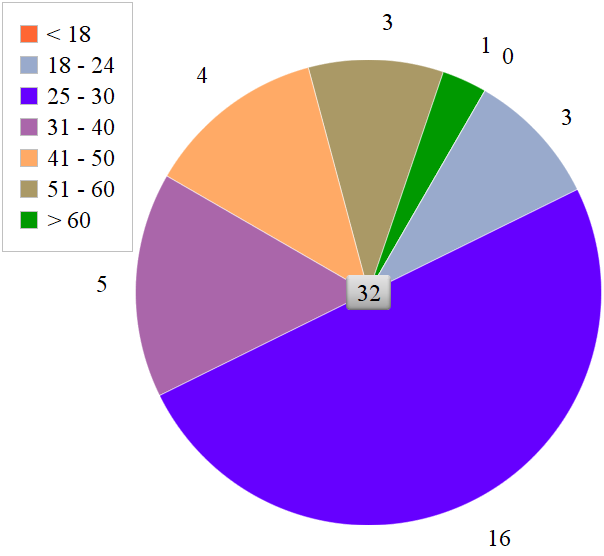
\includegraphics[width=.75\textwidth]{results_agegroups.png}\\ % PNG-File
	\caption{Age distribution of participants in the user study}
	\label{fig:results_agegroups}
\end{figure}

\begin{figure}[htb]
	\centering
	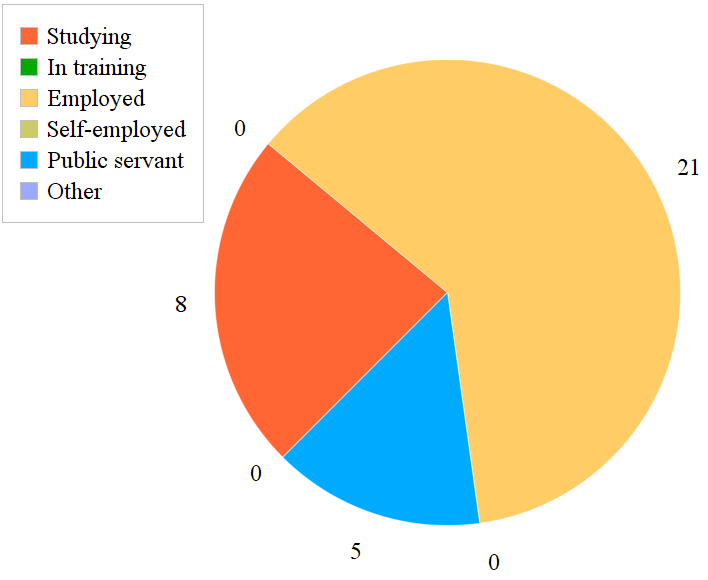
\includegraphics[width=.75\textwidth]{results_working_situation.png}\\ % PNG-File
	\caption{Working situation of participants in the user study}
	\label{fig:results_working_situation}
\end{figure}

The majority of participants was employed and between 25 and 30 years of age.

	\section{Feedback from the questionnaire}
	\label{sec:results_feedback_from_questionnaire}

As described in section \ref{sec:questionnaire}, at the endof the user study, participants were asked to rate a set of statements on a Likert-scale. Figure \ref{fig:feedback_questionnaire} shows the data gathered from this questionnaire. If a user ticked \textit{No comment} for a statement, it was not considered for these average values. The statements are shortened in this figure, the full wording can be found in \ref{sec:questionnaire} as well as appendix 
% @TODO Das mit dem Anhang!

\begin{figure}[htb]
	\centering
	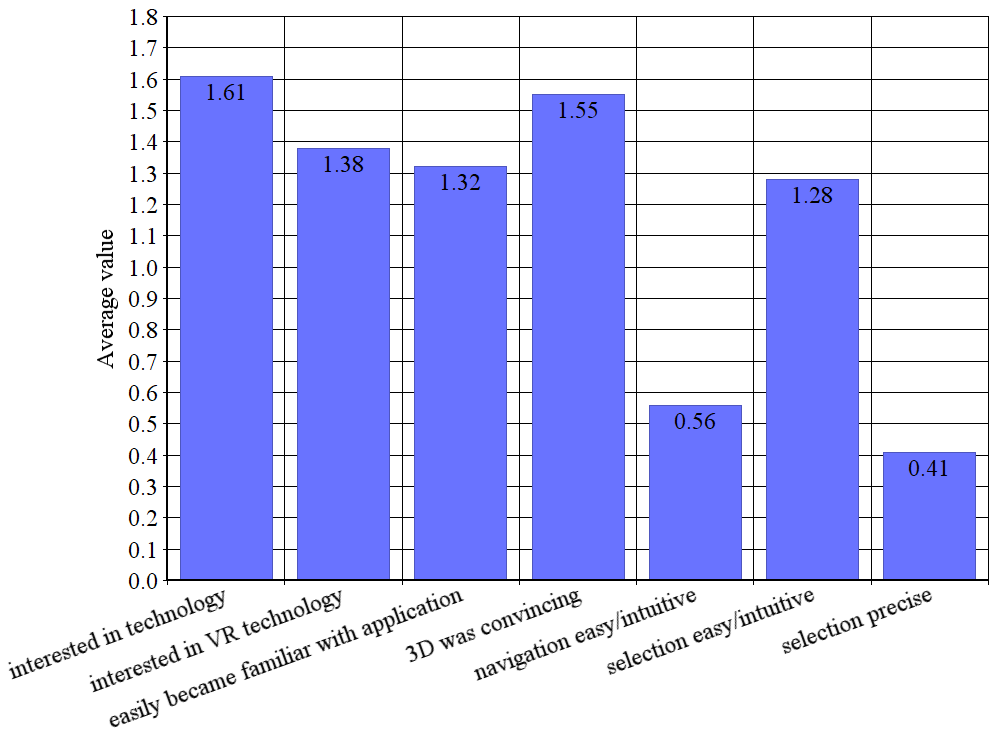
\includegraphics[width=.95\textwidth]{feedback_v2.png}\\ % PNG-File
	\caption{Feedback on the application gathered from the questionnaire. \textit{No comment} answers are not considered.}
	\label{fig:feedback_questionnaire}
\end{figure}

Figure \ref{fig:feedback_questionnaire} shows the average rating of statements on the questionnaire. Answers count as follows.

\begin{enumerate}
	\item \textit{I strongly disagree}: 2
	\item \textit{I disagree}: 1
	\item \textit{No comment}: 0
	\item \textit{I agree}: -1
	\item \textit{I strongly agree}: -2
\end{enumerate}.

Especially the precision of the selection process seemed to be not quit satisfactory to a lot of users. While the average result is still \textit{positive}, 

	\section{Individual feedback and comments}
	\label{sec:individual_feedback_and_comments}
% detailliert Rückmeldungen beschreiben (sieheh Ticket 05.09.17)

	\section{Saliency and difference maps}
	\label{sec:saliency_and_difference_maps}
This section contains figures depicting \textit{mesh saliency} and \textit{user saliency} maps for each object as well as \textit{unweighted} (raw) and \textit{weighted} difference maps. For each object, these maps are shown in three angles, front, side and top. All figures are orthographic renderings. The scale shown in figure \ref{fig:results_scale} is used for all figures. Note that it is uniform in the sense that the color mapping represents values between 0.0 and 1.0. For saliency maps, this expresses the saliency (the \textit{perceived importance} per vertex), for difference maps it expresses the differenc between saliency maps vertex wise.

\begin{figure}[htb]
	\centering
	
\includegraphics[width=.7\textwidth]{result_maps/scale_values.png}\\ % PNG-File
	\caption{The uniform scale used for figures in this section.}
	\label{fig:results_scale}
\end{figure}


		\subsection{Bunny}
		\label{sec:results_bunny}
%
%	BUNNY
%
\begin{figure}[htb]
	\centering
	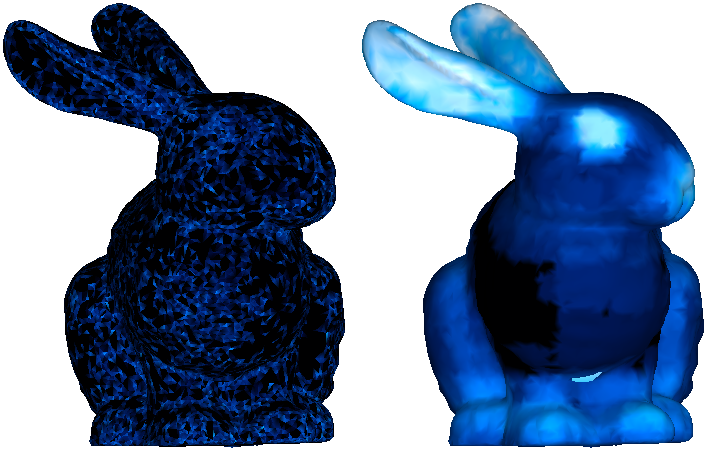
\includegraphics[width=.7\textwidth]{result_maps/bunny/bunny_front_A.png}\\ % PNG-File
	\caption{Normalised saliency maps for the first model, orthographic front view. Left: \textit{mesh saliency}, right: \textit{user saliency}.}
	\label{fig:results_bunny_front_a}
\end{figure}
\begin{figure}[htb]
	\centering
	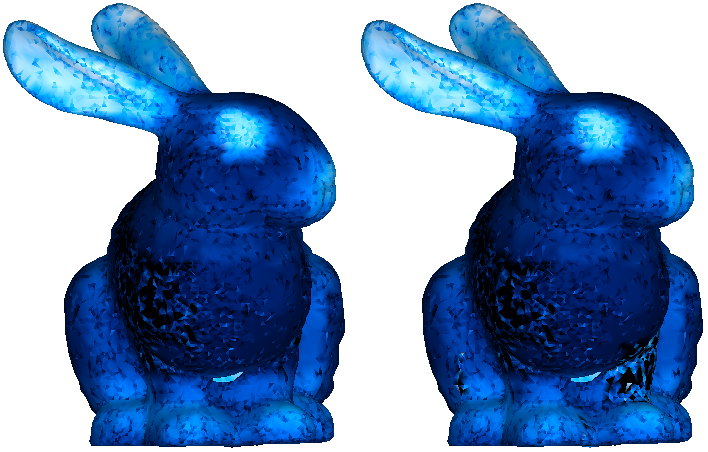
\includegraphics[width=.7\textwidth]{result_maps/bunny/bunny_front_B.png}\\ % PNG-File
	\caption{Normalised difference maps for the first model, orthographic front view. Left: \textit{unweighted differences}, right: \textit{weighted differences}.}
	\label{fig:results_bunny_front_b}
\end{figure}

\begin{figure}[htb]
	\centering
	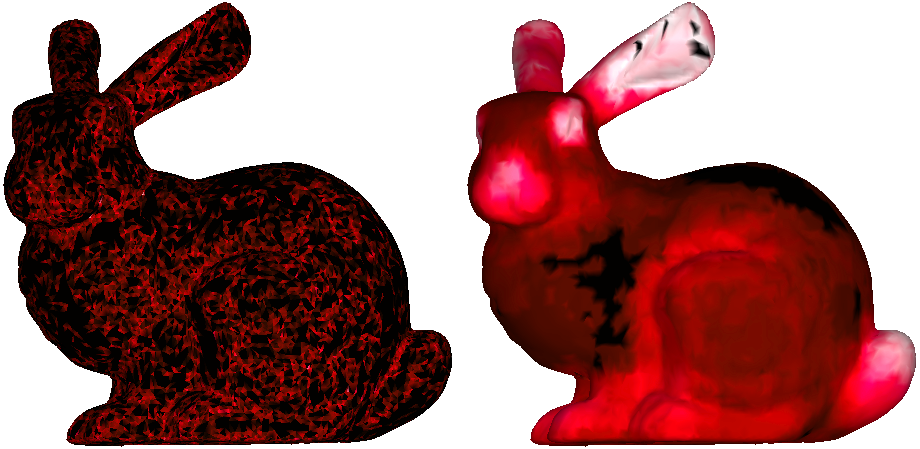
\includegraphics[width=.85\textwidth]{result_maps/bunny/bunny_side_A.png}\\ % PNG-File
	\caption{Normalised saliency maps for the first model, orthographic side view. Left: \textit{mesh saliency}, right: \textit{user saliency}.}
	\label{fig:results_bunny_side_a}
\end{figure}
\begin{figure}[htb]
	\centering
	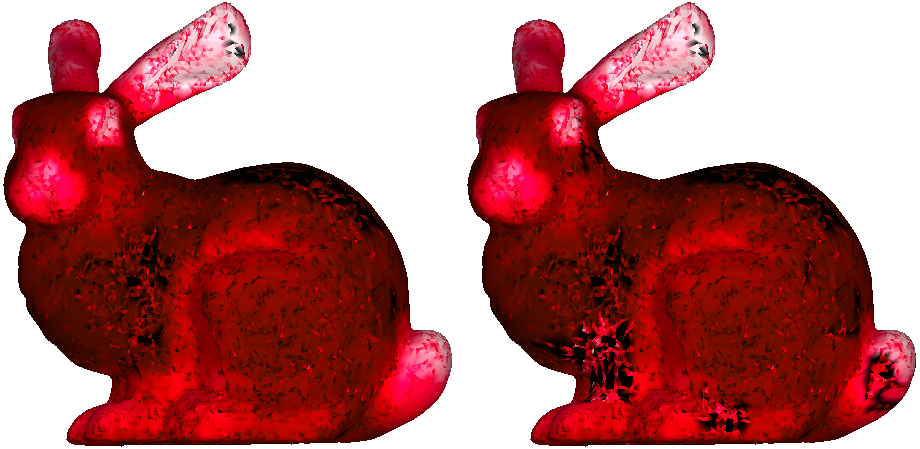
\includegraphics[width=.85\textwidth]{result_maps/bunny/bunny_side_B.png}\\ % PNG-File
	\caption{Normalised difference maps for the first model, orthographic side view. Left: \textit{unweighted differences}, right: \textit{weighted differences}.}
	\label{fig:results_bunny_side_b}
\end{figure}

\begin{figure}[htb]
	\centering
	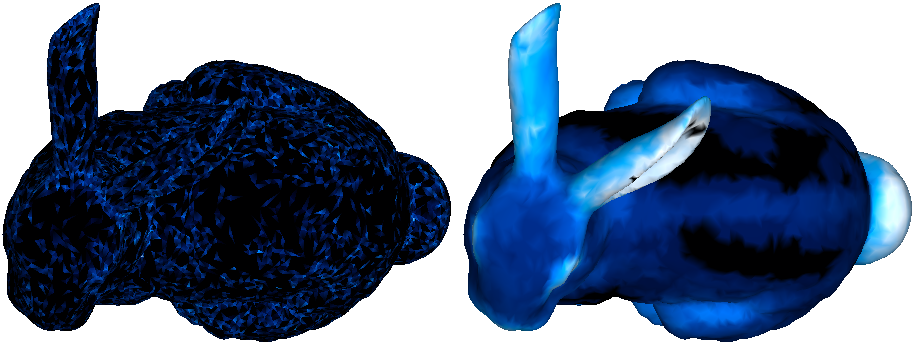
\includegraphics[width=.9\textwidth]{result_maps/bunny/bunny_top_A.png}\\ % PNG-File
	\caption{Normalised saliency maps for the first model, orthographic top view. Left: \textit{mesh saliency}, right: \textit{user saliency}.}
	\label{fig:results_bunny_top_a}
\end{figure}
\begin{figure}[htb]
	\centering
	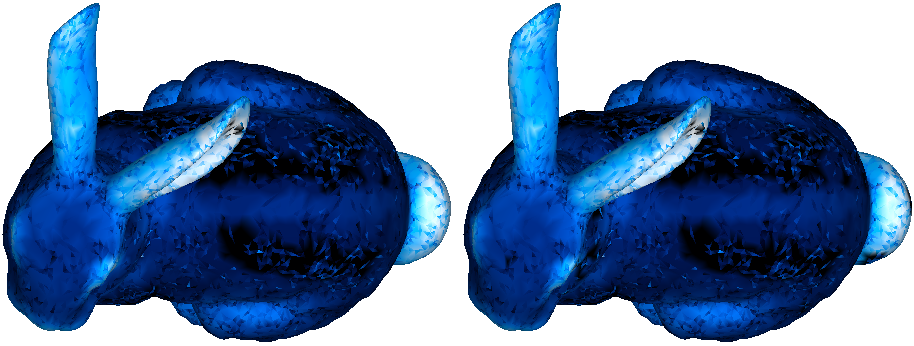
\includegraphics[width=.9\textwidth]{result_maps/bunny/bunny_top_B.png}\\ % PNG-File
	\caption{Normalised difference maps for the first model, orthographic top view. Left: \textit{unweighted differences}, right: \textit{weighted differences}.}
	\label{fig:results_bunny_top_b}
\end{figure}

		\subsection{Cow}
		\label{sec:results_cow}
%
%	COW
%
\begin{figure}[htb]
	\centering
	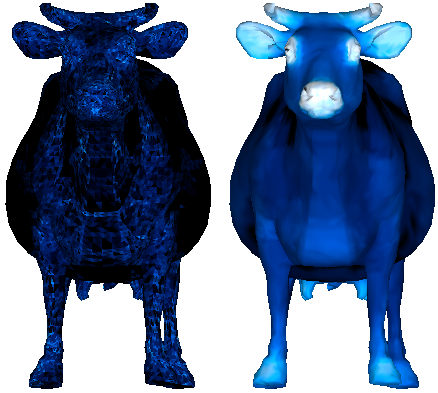
\includegraphics[width=.55\textwidth]{result_maps/cow/cow_front_A.png}\\ % PNG-File
	\caption{Normalised saliency maps for the second model, orthographic front view. Left: \textit{mesh saliency}, right: \textit{user saliency}.}
	\label{fig:results_cow_front_a}
\end{figure}
\begin{figure}[htb]
	\centering
	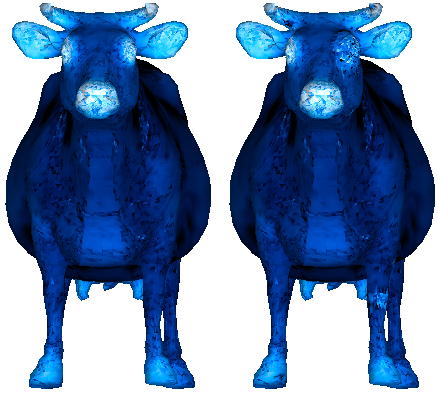
\includegraphics[width=.55\textwidth]{result_maps/cow/cow_front_B.png}\\ % PNG-File
	\caption{Normalised difference maps for the second model, orthographic front view. Left: \textit{unweighted differences}, right: \textit{weighted differences}.}
	\label{fig:results_cow_front_b}
\end{figure}

\begin{figure}[htb]
	\centering
	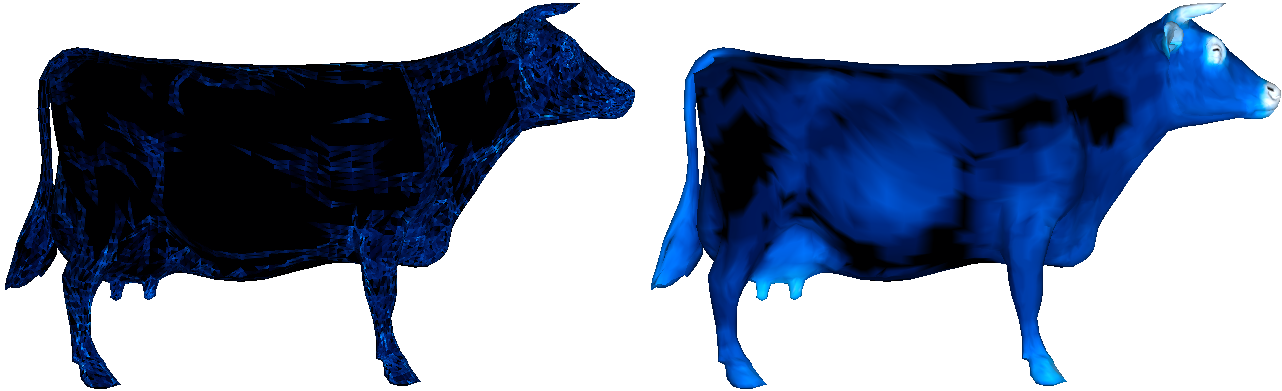
\includegraphics[width=1.0\textwidth]{result_maps/cow/cow_side_A.png}\\ % PNG-File
	\caption{Normalised saliency maps for the second model, orthographic side view. Left: \textit{mesh saliency}, right: \textit{user saliency}.}
	\label{fig:results_cow_side_a}
\end{figure}
\begin{figure}[htb]
	\centering
	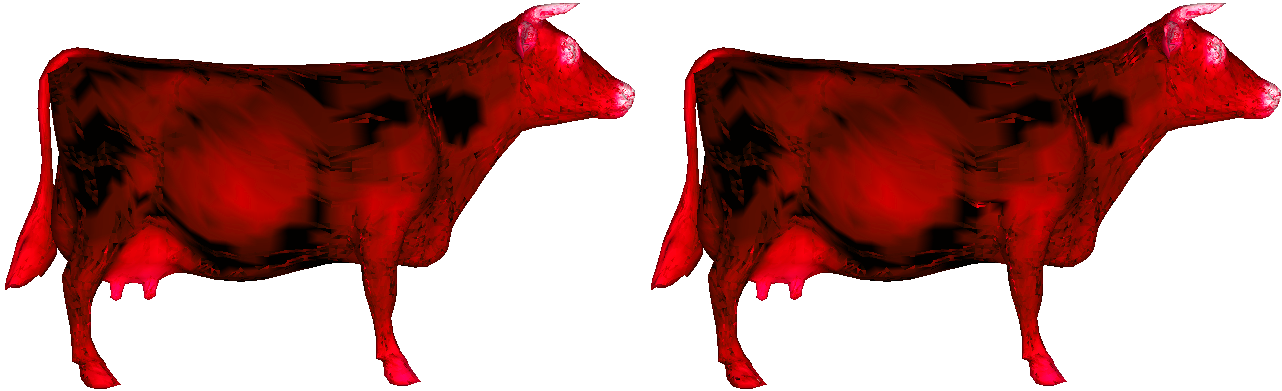
\includegraphics[width=1.0\textwidth]{result_maps/cow/cow_side_B.png}\\ % PNG-File
	\caption{Normalised difference maps for the second model, orthographic side view. Left: \textit{unweighted differences}, right: \textit{weighted differences}.}
	\label{fig:results_cow_side_b}
\end{figure}

\begin{figure}[htb]
	\centering
	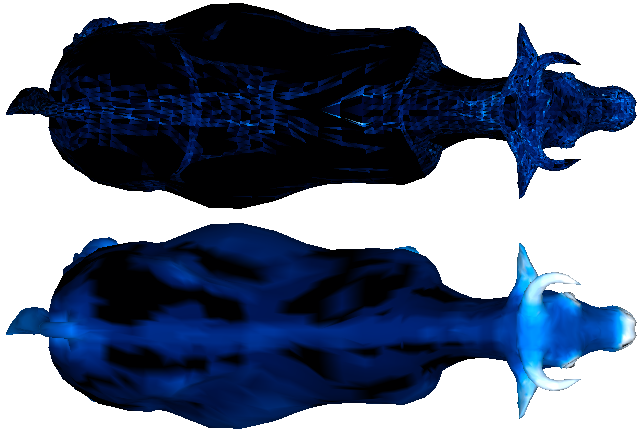
\includegraphics[width=.7\textwidth]{result_maps/cow/cow_top_A.png}\\ % PNG-File
	\caption{Normalised saliency maps for the second model, orthographic front view. Top: \textit{mesh saliency}, bottom: \textit{user saliency}.}
	\label{fig:results_cow_top_a}
\end{figure}
\begin{figure}[htb]
	\centering
	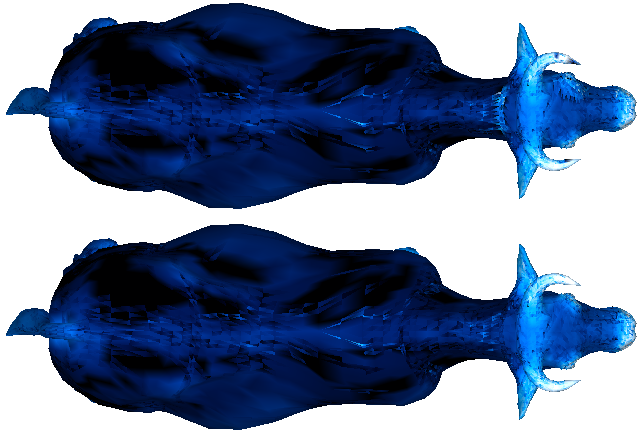
\includegraphics[width=.7\textwidth]{result_maps/cow/cow_top_B.png}\\ % PNG-File
	\caption{Normalised difference maps for the second model, orthographic top view. Top: \textit{unweighted differences}, bottom: \textit{weighted differences}.}
	\label{fig:results_cow_top_b}
\end{figure}

		\subsection{P51}
		\label{sec:results_p51}
%
%	P51
%
\begin{figure}[htb]
	\centering
	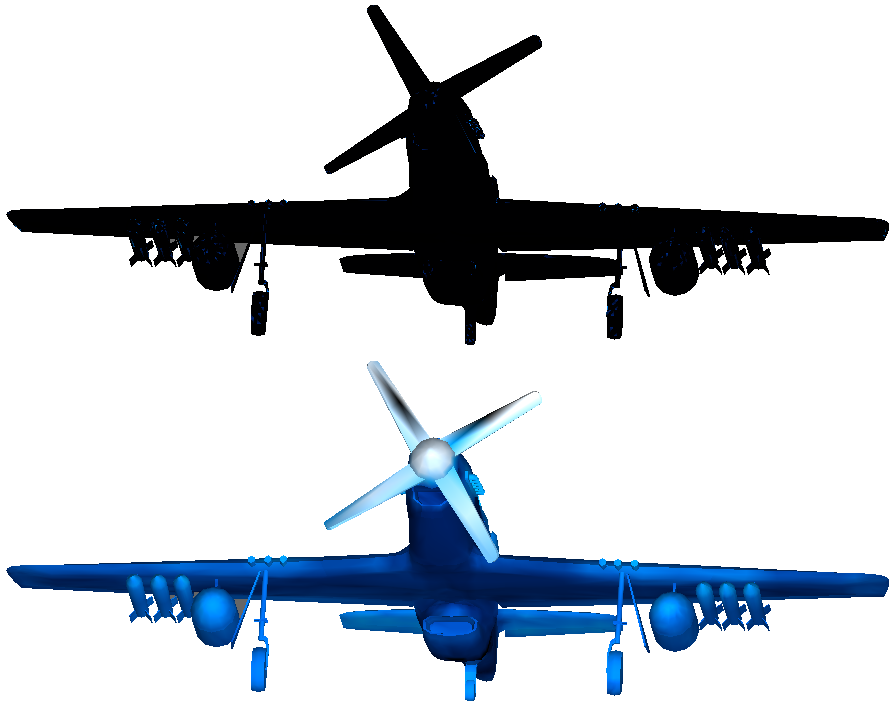
\includegraphics[width=.7\textwidth]{result_maps/P51/P51_front_A.png}\\ % PNG-File
	\caption{Normalised saliency maps for the third model, orthographic front view. Top: \textit{mesh saliency}, bottom: \textit{user saliency}.}
	\label{fig:results_p51_front_a}
\end{figure}
\begin{figure}[htb]
	\centering
	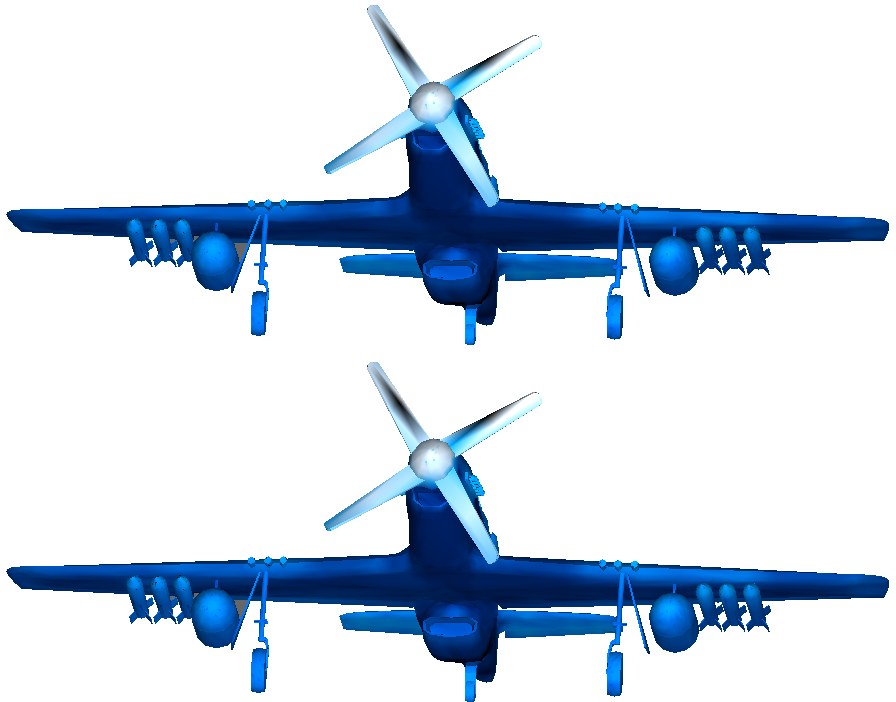
\includegraphics[width=.7\textwidth]{result_maps/P51/P51_front_B.png}\\ % PNG-File
	\caption{Normalised difference maps for the third model, orthographic front view. Top: \textit{unweighted differences}, bottom: \textit{weighted differences}.}
	\label{fig:results_p51_front_b}
\end{figure}

\begin{figure}[htb]
	\centering
	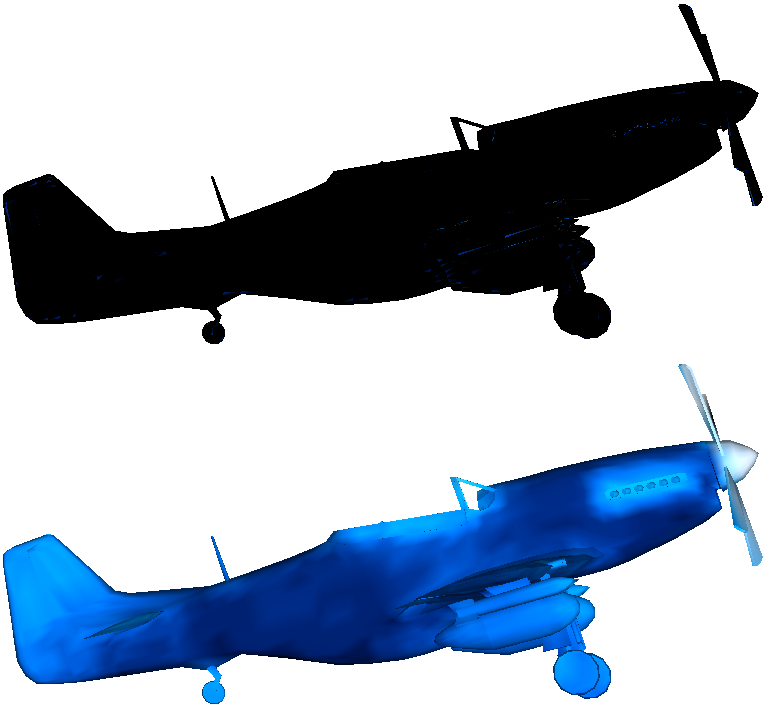
\includegraphics[width=.7\textwidth]{result_maps/P51/P51_side_A.png}\\ % PNG-File
	\caption{Normalised saliency maps for the third model, orthographic side view. Top: \textit{mesh saliency}, bottom: \textit{user saliency}.}
	\label{fig:results_p51_side_a}
\end{figure}
\begin{figure}[htb]
	\centering
	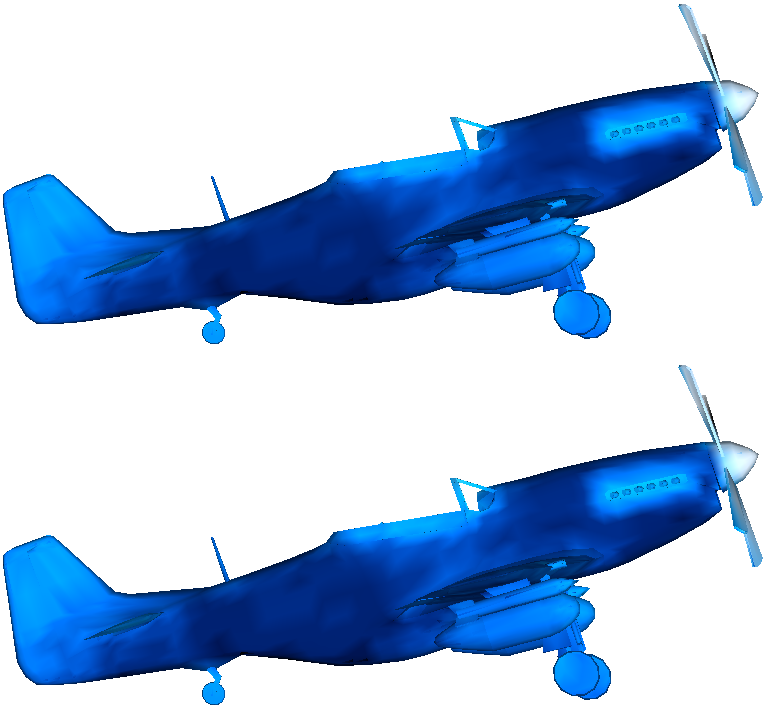
\includegraphics[width=.7\textwidth]{result_maps/P51/P51_side_B.png}\\ % PNG-File
	\caption{Normalised difference maps for the third model, orthographic side view. Top: \textit{unweighted differences}, bottom: \textit{weighted differences}.}
	\label{fig:results_p51_side_b}
\end{figure}

\begin{figure}[htb]
	\centering
	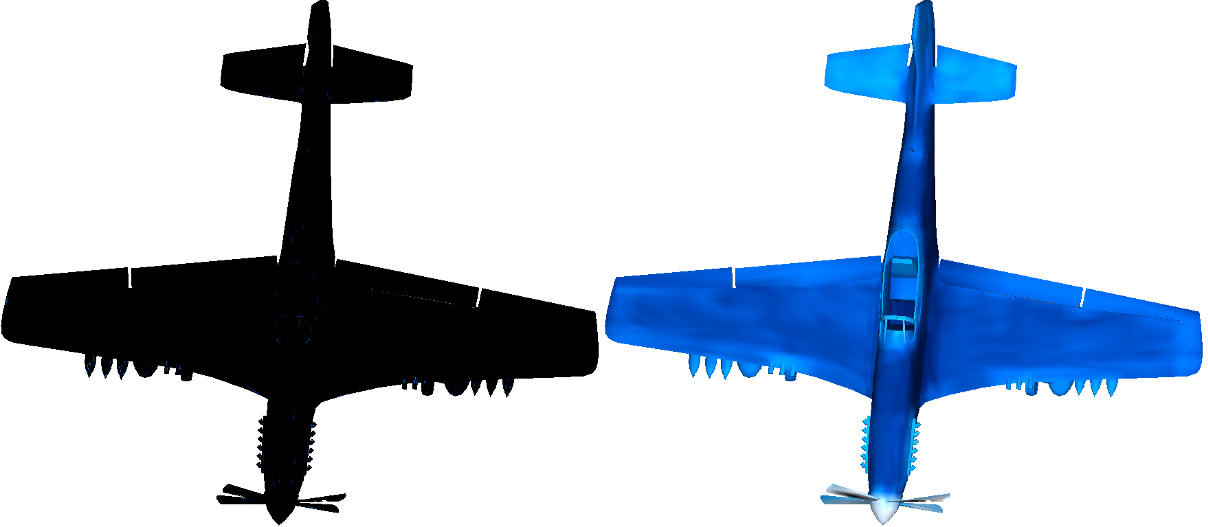
\includegraphics[width=.9\textwidth]{result_maps/P51/P51_top_A.png}\\ % PNG-File
	\caption{Normalised saliency maps for the third model, orthographic top view. Left: \textit{mesh saliency}, right: \textit{user saliency}.}
	\label{fig:results_p51_top_a}
\end{figure}
\begin{figure}[htb]
	\centering
	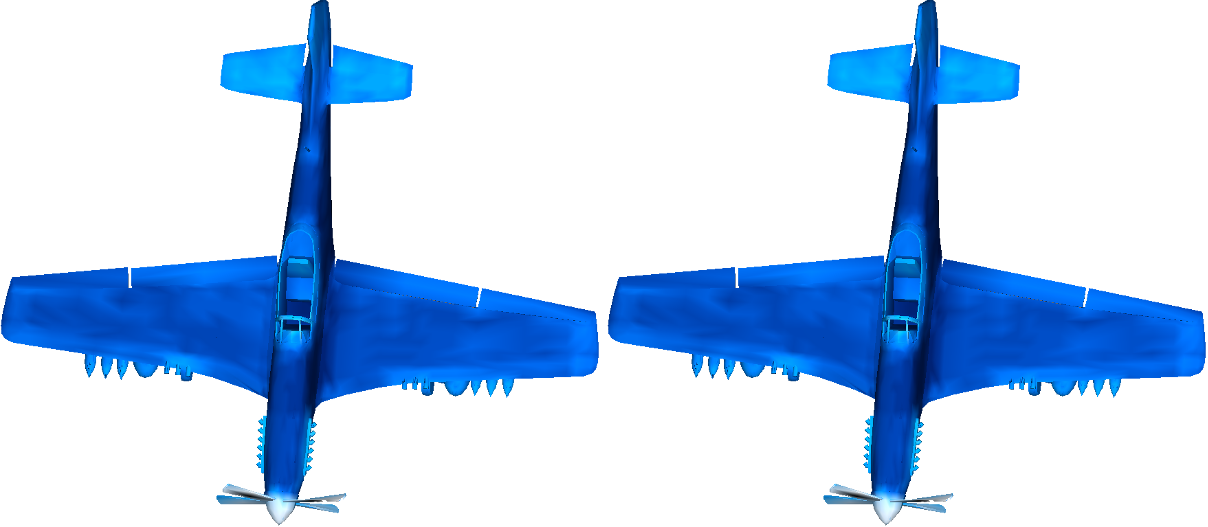
\includegraphics[width=.9\textwidth]{result_maps/P51/P51_top_B.png}\\ % PNG-File
	\caption{Normalised difference maps for the third model, orthographic top view. Left: \textit{unweighted differences}, right: \textit{weighted differences}.}
	\label{fig:results_p51_top_b}
\end{figure}
%
%	ENDE BILDER
%

	\section{Evaluation of differences}
	\label{sec:evaluation_of_differences}

		\subsection{Measure of difference}
		\label{sec:measure_of_difference}

		\subsection{Observation of saliency maps}
		\label{sec:observation_of_saliency_maps}

		\subsection{Mesh saliency with mechanical objects}
		\label{sec:mesh_saliency_with_mechanical_objects}

